\documentclass[12pt,letterpaper]{article}
\usepackage{geometry}
\usepackage[utf8]{inputenc}
\usepackage{natbib}
\usepackage{lscape}
\usepackage{amsmath}
\usepackage{amsfonts}
\usepackage{amssymb}
\usepackage{graphicx}
\usepackage{subfig}
\usepackage{float}
\usepackage{algpseudocode}
\usepackage{fancyhdr}
\usepackage{comment}
\usepackage{hyperref}

\usepackage[english]{babel}
\geometry{verbose,letterpaper,tmargin=3cm,bmargin=3cm,lmargin=2.5cm,rmargin=2.5cm}

% Tables
\usepackage{multirow}
\usepackage[table]{xcolor}

% Avoid to split words at the end of each line
\usepackage{hyphenat}

\usepackage{setspace}

\usepackage{natbib} 
\setcitestyle{numbers,square}

\usepackage{notoccite}


\singlespacing

\begin{document}

% BEGIN TITLE PAGE
\begin{titlepage}

\Large
\sffamily

\begin{center}
  \begin{tabular}{c}
    
\includegraphics[width=0.30\textwidth]{logo-eafit.png}
  \end{tabular}
\end{center}

\vfill
\begin{center}
  \LARGE Deep learning techniques for Blood Flow simulation based on Navier-Stokes Equations
\end{center}

\vspace*{1cm}
\centerline{\LARGE Alejandro Salazar Arango\footnotemark}  
\footnotetext{Mathematical Engineering Student. Universidad EAFIT asalazara1@eafit.edu.co}
\vfill

\begin{center}
Advisor(s): \\
Cristhian David Zambrano Mora\footnote{School of Applied Sciences and Engineering. Universidad EAFIT cdmontoyaz@eafit.edu.co}   \\
\end{center}

\vfill

\begin{center}
  \large
    Research practice 3 \\
  Research proposal \\
  Mathematical Engineering\\
  School of Applied Sciences and Engineering\\
  Universidad EAFIT \\
\end{center}

\vfill
\centerline{August 2023}
\vspace*{0.7cm}
\end{titlepage}

% END TITLE PAGE

\section{Introduction}

\begin{comment}

  (\textcolor{red}{4 a 5 párrafos})

Debe incluir:

\begin{itemize}
\item Contexto corto para ubicar al lector.
\item Corta descripción del problema u oportunidad de investigación.
\item Aporte de la investigación.
\item Párrafo que justifique la importancia de la investigación.
\end{itemize}

\end{comment}

Partial differential equations (PDEs) are one of the most powerful tools for the study of physical and biological phenomena. They allow us to represent in a simplified way, the dynamics between the spatial and temporal variables of any phenomenon and to take these dynamics to a mathematical model, whose solution describes in a great way the behavior of the studied system\cite{logan2014applied}. This has led partial differential equations to become a tool of great use in areas such as fluid dynamics, electromagnetism, optics, magnetism, among others\cite{farlow1993partial}; these areas being dominated by PDEs such as Maxwell's Equations and Navier-Stokes Equations, the latter being the object of study of the present work. \\

However, PDEs, given their complex structure, are usually models whose analytical solutions are difficult or impossible to find, being even the solutions already found for some PDEs so complex that it is preferred to use other methods to solve the problem\cite{strauss2007partial}. This is why, in recent years, the development of multiple numerical methods to solve this type of equations has been one of the major topics of study of the scientific community. In addition, numerical methods for solving PDEs are a really important topic of study given that although there are already multiple methods developed, if these are not applied correctly can lead to solutions far from the real solution of the problem and therefore lead to erroneous conclusions about the behavior of the system under study.\\

One of the most commonly used numerical method for solving Partial Differential Equations is the Finite Element Method (FEM), a numerical method consisting on the discretization of the problem's domain, to later solve a variational formulation of the problem with determined test functions, to obtain an algebraic system of equations, which, when solved, gives the approximated solution of the problem. However, due to the substantial number of degrees of freedom it needs in order to correctly solve the PDE, it remains as an extremely expensive method both in terms of CPU and memory demand, therefore not being too useful for real-time contexts\cite{hesthaven2018non} \cite{PINNQuarteroni}. Consequently, models such as reduced basis models (RBMs) and physically informed neural networks (PINNs) have been developed and have become important methods in the study of PDEs.\\

This project focuses on the implementation of artificial intelligence models for the solution of PDEs, specifically Physical Informed Neural Networks (PINNs) and Neural Network assisted Reduced Basis Models (NN-RBM), seeking to obtain a reduced computational cost in a real-time simulation context. The Navier-Stokes equations, and in particular, a simulation problem of blood flow through the carotid artery, will be used as an object of study, to observe and compare the performance of these methods versus the FEM in an on-line simulation process, aiming for a deeper understanding of the advantages and limitations of NN-RBMs, PINNs and FEM in the context of real-time simulations.


\begin{comment}
  Parrafo comentando los principales métodos implementados en CFD (principamente FEM) comentar el alto número de grados de libertad e introducir RBM y PINN utilizando NN.
  
  Parrafo comentando rápidamente el objetivo de la investigación, como se realizará y el aporte esperado.
\end{comment}

\section{Statement of the problem}



\subsection{Statement of the problem}

\begin{comment}
  \textcolor{red}{4 a 5 párrafos})
  En este apartado debemos ampliar la descripción del problema.

  En esta subsección se hace una ampliación del problema descrito en la introducción. Acá hay
  algunas aspectos que se pueden abordar acá.

  \begin{itemize}
 \item En algunos casos, un problema tiene diferentes nombres en la literatura. En estos casos es bueno contarle al lector con qué otros nombre se conoce el problema en diferentes áreas de conocimiento.
 \item Si es una investigación aplicada, es conveniente pensar en que matices o particularidades adquiere el problema al aplicarse en un contexto específico. Puede que lo que no sea un problema en un lugar si lo sea en otro.
 \item ¿A quienes afecta el problema?¿a qué escala opera? (grupos poblacionales, zonas geográficas, período temporal: pasado, actual o futuro).
 \item ¿Qué desencadena o genera el problema?
 \item ¿Qué repercusiones o efectos tiene el problema?
 \item ¿Se han postulado soluciones a este problema pero no lo suficientemente satisfactorias?
\end{itemize}

\end{comment}


For solving fluid dynamics problems, Computational Fluid Dynamics (CFD) uses three methods: The Finite Difference Method, The Finite Volumes Method, and the Finite Element Method.  In the finite volume method, the discretization is performed by partitioning the spatial domain into a mesh, in which each of its elements will be called a control volume. The idea is to perform the integration of the dominant equations of the problem through each control volume, balancing the fluxes across the boundaries of the individual volumes and getting what is called a balance equation. Then the set of balance equations will be discretized with respect to a set of discrete unknowns to finally get the solution to the problem\cite{volumes}. In a topologically regular mesh, these calculations are done quite easily, but when working with irregular meshes, this calculation will result in an unbearable amount of fluxes and a significant accounting effort to ensure that all fluxes have been calculated correctly\cite{AutoDesk}.\\

In the finite difference method, the derivatives of the problem are usually replaced by truncated expansions of the Taylor series, this method is straightforward for regular geometries, but when working with irregular geometries it is necessary to perform transformations to the equations before the expansion is carried out\cite{AutoDesk}. Finally, the finite element method works by dividing the initial domain of the same (a continuous element) into a large number of non-intersecting subdomains, called finite elements. At last, the formulation of a boundary value problem ends up giving a system of algebraic equations, which are then solved using variational methods to approximate a solution, minimizing an associated error function\cite{element}. Nevertheless, these approaches come with a significant drawback. Due to their extensive equation systems, they demand a substantial number of degrees of freedom to accurately approximate the model solution. \\


This becomes a problem because as the complexity of the problem increases, the number of degrees of freedom will also increase and this, in turn, means that for the model to be solved correctly, a greater use of computational resources such as memory, storage and processing capacity will be necessary. This implies that the problem takes more time to solve, reaching a point where even the available resources may be insufficient to solve the problem properly. Because of the above, the commonly used models do not excel as efficient choices for a real-time context and given the importance of a fast response rate in some of the applications of PDEs\cite{raissi2019physics}, it becomes important to develop new agile methods for the solution of PDEs.\\

In this regard, one of the main solutions proposed in the literature are the Reduced Base Models (RBM), which base their solution process on two phases, in a first offline phase, a group of representative snapshots  of the model's parameter space is obtained and from this a reduced base of the space is built, to later, in a second online phase, project the complete order system on this reduced base, and thus obtain an approximate solution of the problem as a linear combination of the elements of the base. However, this method does not represent much computational gain when the problems are overly complex, since this leads to the projection process being equally complex and therefore does not allow the correct solution of the PDE in the expected time.


\subsection{Formalization of the problem}

\begin{comment}
  En esta subsección debén escribir una descripción más formal, muy al grano,
del problema.  Se deben incluir los principales elementos matemáticos que
tiene el problema.  En la siguiente figura hay un ejemplo de formalización del
problema tomado de Duque, J. C., Anselin, L., \& Rey, S. J. (2012). The
max‐p‐regions problem. Journal of Regional Science, 52(3), 397-419.


 \begin{center}
  \begin{tabular}{c}
    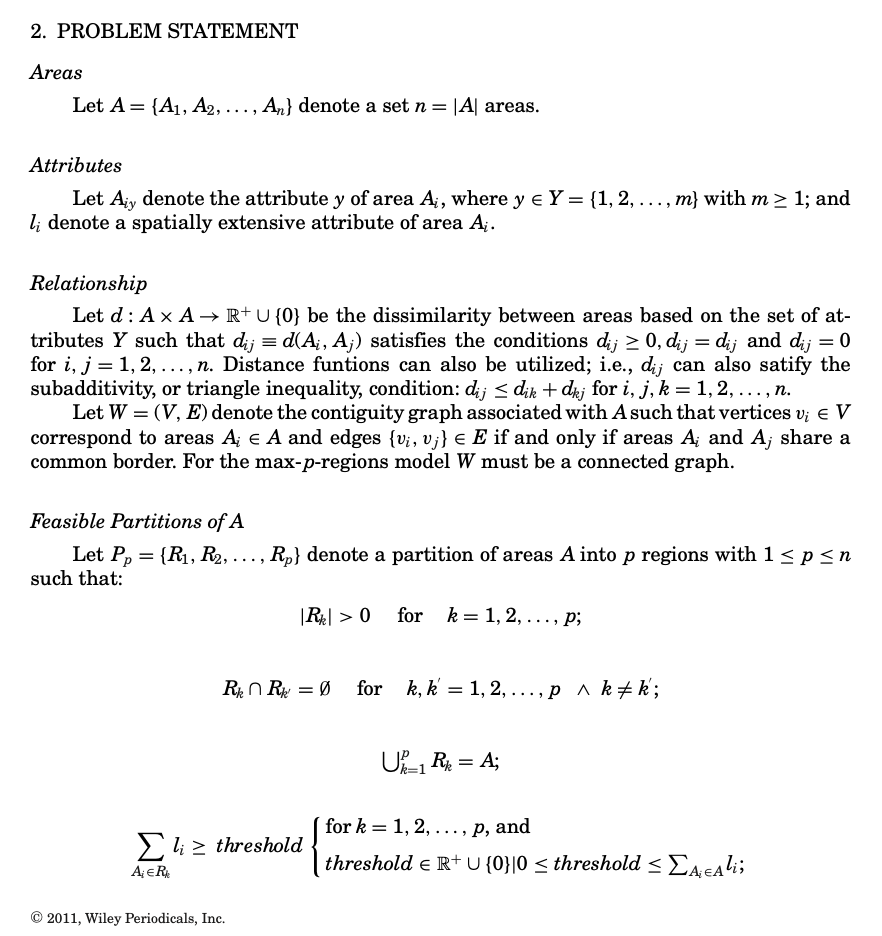
\includegraphics[width=0.70\textwidth]{problem_statement}
  \end{tabular}
\end{center}

\end{comment}

In a domain $\Omega\subset \mathbb{R}^2$  Quateroni\cite{quarteroni2009numerical} 
define incompressible Navier-Stokes Equations as follows 

\begin{equation}
  \begin{cases}
     \nabla \cdot \textbf{u} = 0 & \textbf{x} \in \Omega , t > 0\\
     
     \textbf{u}_t - \nabla \cdot[\nu (\nabla \textbf{u} + \nabla \textbf{u}^T)] + (\textbf{u}\cdot \nabla)
     \textbf{u}+ \nabla p = \textbf{f} & \textbf{x} \in \Omega , t > 0
  
  \end{cases}
  \label{1}
\end{equation}\\

When $\nu$ is constant, we obtain

$$\nabla \cdot[\nu (\nabla \textbf{u} + \nabla \textbf{u}^T)] = \nu (\Delta \textbf{u} + \nabla(\nabla \cdot \textbf{u})) = \nu \Delta \textbf{u}$$

and therefore the equations are written as

\begin{equation}
  \begin{cases}
     \nabla \cdot \textbf{u} = 0 & \textbf{x} \in \Omega , t > 0\\
     
     \textbf{u}_t - \nu \Delta \textbf{u} + (\textbf{u}\cdot \nabla)
     \textbf{u}+ \nabla p = \textbf{f} & \textbf{x} \in \Omega , t > 0
  
  \end{cases}
  \label{2}
\end{equation}\\

Being $\textbf{u}$ the fluid velocity field, $p$ the pressure divided by the density $\rho$, $\nu$
the kinematic viscosity define as $\frac{\mu}{\rho}$ with $\mu$ being the dynamic viscosity and $\textbf{f}$ 
a forcing term per unit mass.\\~\\
For the purpose of this work the domain $\Omega$ must also be bounded, and it is therefore necessary 
to assign initial and suitable boundary conditions for the problem to be well posed.

$$\begin{cases}
  \textbf{u}(\textbf{x},0) = \textbf{u}_0(\textbf{x}) & \forall \textbf{x} \in \Omega \\
  \textbf{u}(\textbf{x},t) = \varphi(\textbf{x},t) & \forall \textbf{x}\in \varGamma_D, t>0 \\
  \left(\nu\frac{\partial \textbf{u}}{\partial \textbf{n}}-p\textbf{n}\right)(\textbf{x},t) = \psi(\textbf{x},t) & \forall \textbf{x}\in \varGamma_N, t>0

\end{cases}$$

Where $\textbf{u}_0$ is a divergence free vector field,  $\varphi$ and $\psi$ are given vector
functions, $\varGamma_D$ and $\varGamma_N$ provide a partition of the boundary $\partial \Omega$ and 
\textbf{n}, as usual, represents the outward unit normal vector to $\partial \Omega$.


\section{Objectives}

\subsection{General objective}

\begin{comment}
  (\textcolor{red}{sólo uno})
  El objetivo general enmarca todo el trabajo. Está estrechamente relacionado con el
título y con la pregunta de investigación y describe de intensión de la
invesstigación.

La estructura de un objetivo general es la siguiente: verbo en infinitivo (uno
solo) + qué (objeto de estudio) + cómo + para qué.
\end{comment}

Compare the performance of Neural Network assisted Reduced Basis Models (NN-RBMs) and Physical Informed Neural Networks (PINNs) against the Finite Element Method on a real-time context, by performing multiple simulations of the blood flow through the carotid artery.

\subsection{Specific objectives}

\begin{comment} 
  (\textcolor{red}{3 o 4 objetivos})
  Son un conjunto de objetivos más pequeños que permitirán alcanzar el general.
  La estructura de un objetivo general es la siguiente: Verbo en infinitivo (uno
  solo) + qué (objeto de estudio) + cómo.

  Importante: los objetivos específicos no se pueden confundir con una lista de
  tareas. El objetivo debe comenzar con un fin/logro no con el medio/actividad
  (las actividades van en la metodología); por ejemplo, un objetivo específico
  del tipo ``Realizar una revisión bibliográfica para...'' debería transformarse
  en algo como ``Encontrar información científica por medio de una revisión
  sistemática de la literatura''.

\end{comment}

\begin{itemize}
  \item Identify the principal differences on the implementation of NN-RBMs and PINN like models and FEM in a fluid mechanic context.
  \item Assess the ability of NN-RBMs and PINNs to adapt to changing boundary conditions or parameters, compared to the FEM approach.
  \item  Study the generalization capabilities of NN-RBMs and PINNs when trained on a specific set of data and tested on different scenarios, compared to FEM.
  \item Analyze the dependency of NN-RBMs to the Snapshots used for the training on the model
\end{itemize}

\section{Justification}

\begin{comment}

En esta sección se argumenta el por qué es importante resolver el problema o
contestar la pregunta de investigación. Las argumentaciones pueden ser de tipo
teórico o práctico y soportadas en literatura.

\begin{itemize}
\item Destaca los beneficios derivados del aporte (¿para qué servirá esta investigación?, ¿qué aporta de nuevo esta investigación?, ¿cuáles son los beneficios?, ¿quiénes serán los beneficiados y de qué modo?, ¿qué se prevé cambiar con la investigación?, ¿cuál es la utilidad?, ¿resolverá algún problema práctico?, ¿se cubrirá algún gap de conocimiento?, ¿los resultados se podrán generalizar?, ¿sirve para apoyar alguna teoría?, ¿permite un mejor estudio de una población o fenómeno?, ¿se pueden establecer plazos para los beneficios?). OJO: las preguntas no se incluyen en el cuerpo del texto, son sólo una guía para encontrar los argumentos.
\item Las respuestas a estas preguntas deben considerar tres aspectos: teórico, práctico y metodológico.
\end{itemize}

\end{comment}

As previously mentioned, PDEs are one of the most powerful tools used in multiple fields for the modeling of dynamic systems, however, given their applications in fields such as electromagnetism, fluid dynamics and heat transfer, given the nature of the problem to be solved, it is often necessary to process the model online to provide a quick response to the conditions encountered. This is why, given the high computational cost of the usual numerical methods, it is necessary to implement new models based on computational tools and techniques that allow us to speed up the solution process and, therefore, give an answer to the problem posed.\\

Now, speaking specifically of the Navier-Stokes equations, these are usually some of the equations that can bring more complications when solving, because, although it is common to see works in which simulations of the solutions of these equations are performed using FEM methods, these equations are still equations with a high level of complexity, and if we include the irregularity of the domains over which it is possible to simulate the flow of a fluid (such as blood, which is used in the present work), it becomes a problem of high complexity, which although it can be solved using more traditional methods, can take considerable time to solve and therefore, the use of methods such as PINNs and NN-RBMs can imply a significant improvement in the solution process.\\

PINNs are quite useful in this type of problems since, by incorporating the physical information of the system under study in the training of the neural networks, allowing the imposition of boundary conditions and governing equations directly on the network architecture, it facilitates the adaptation of the network to different conditions and geometries on which to solve the problem, in addition to potentially even improving the accuracy of the numerical solutions.\\

Finally, on the side of NN-RBMs, they combine two extremely useful approaches in the solution of PDEs, combining the computational power of neural networks with the representation power of RBMs. By means of this, the NN-RBMs not only fulfill their mission of reducing the order of the space on which the problem is worked, but also, by incorporating the neural networks in the process of projection of the system on the reduced basis, they allow to considerably accelerate the process of solution of the PDEs and, therefore, they show an interesting balance between the precision of the model and the speed of response of the same one.


\section{Scope}

\begin{comment}
  \textcolor{red}{2 o 3 párrafos})

  Describe las principales barreras o limitaciones de la investigación,
  así como las principales herramientas y otros recursos que esperaba utilizar
  durante la ejecución del proyecto. También describe los principales
  resultados esperados de la investigación
\end{comment}

The main focus of this project is a theoretical-practical approach, which seeks not only to implement the aforementioned models, but also to review the theoretical bases on which they are constructed, aiming to contribute to a deeper understanding of the advantages and limitations of NN-RBMs, PINNs and FEM in the context of real-time simulations of the Navier-Stokes equations, as well as the mathematical explanation of why they work so well on the presented problem; guiding researchers and practitioners in selecting the most appropriate method for specific applications based on accuracy, computational efficiency and mathematical considerations.\\

Now then, it is clear that for this kind of project one of the biggest obstacles that it is possible to encounter when researching and implementing the model is the impossibility of carrying out analytical validation of the solution obtained by the method, since as it is known, the Navier-Stokes equations, due to their high complexity, do not have an analytical solution against which to compare the numerical solution. However, since multiple models are implemented, and having the FEM as a commonly accepted method for the solution of Parameterized PDEs, it's solution will be used as an accepted solution for validating the implemented models.


\section{State of the art}

\begin{comment}
(\textcolor{red}{5 a 6 párrafos})
Describe las principales referencias relacionadas con el problema. Este estado
del arte puede referirse al problema o aplicación específica, o bien a los
métodos aplicados para solucionarlo. No debes olvidar incluir los trabajos más
importantes y los más recientes.

\end{comment}

Given its important on a great amount of biological, medical, and physical fields, PDEs are one of the most studied topics in applied mathematics, and therefore, a large body of literature on the subject can be found. The following is a review of some of the literature consulted on PINNs and RBMs and their applications in EDPs, where a collection of both theoretical and applied papers are presented.\\

As RBM is one of the most prolific methodologies for solving PDEs in recent years, it is not surprising that a large amount of content can be found in the literature. A first example is the paper by Lin \textit{et al} \cite{lin2023dynamic} in which the authors present an order reduction model based on dynamic mode decomposition (DTM) for parameterized time-dependent PDEs, in which, after using a proper orthogonal decomposition (POD) technique, they use DMD to predict the coefficients over a larger region than the training region. Here the authors explain in a detailed way the methods and algorithms used, which really helps the reader on the understanding of the developed method. Likewise, Zhao \& Piao \cite{zhao2023reduced} present the development of a method based on the application of POD to a Galerkin finite element formulation, for the Kerteweg de Vries regularized long-wave Rosenau equation, using, like Lin \textit{et al} \cite{lin2023dynamic}, a rather mathematical approach for the presentation of their results. \\

However, the literature related to RBM does not stop here, but goes further, as there are also studies in which hybrid models are presented using artificial intelligence techniques. One of these examples is the paper by Kutyniok \textit{et al.} \cite{kutyniok2022theoretical}, which presents a theoretical analysis of both RBMs and neural networks, to end their paper making a link between both techniques for the solution of parameterized PDEs. Following this idea, Pichi, Moya \& Hesthaven \cite{pichi2023graph} present an application of Graph neural networks for solving multiple parameterized PDEs in union with a RBM technique. Likewise, authors like Hesthaven \& Ubbiali \cite{hesthaven2018non} and Fresca, Dede \& Manzoni \cite{fresca2021comprehensive} present interesting approach combining neural network with RBM techniques for solving PDEs. \\

On the other hand, although PINNs are new techniques in the solution of PDEs, they have also been shown to be a topic of great interest to the scientific community and therefore it is not difficult to find literature on the subject, not only for forward problems but for inverse problems as well. On this matter, Berg \& Nyström \cite{berg2021neural} , Meng \& Karniadakis \cite{meng2020composite} and Raissi, Perdikaris \& Karniadakis \cite{raissi2019physics} present three works of interest in which they use PINNs as a solution method for inverse problems with multiple examples and making a focus on the explanation of how PINNs work on every presented examples, as well as a mathematical background on the method itself.\\

Some works about the usage of PINN for fluid dynamics problems can be found as well. A first interesting work on this topic can be found in the paper from Moschou \textit{et al.} \cite{moschou2023physics} who present an application of PINNs on the modeling of astrophysical shocks, focusing on the solar termination shock, a phenomenon described using the fluid dynamics conservation laws. In agreement Ciao \textit{et al.} \cite{xiao2023physics} developed an application of PINN for the turbulent mixing induced by the Rayleigh-Taylor instability, using the Reynolds-Averaged Navier–Stokes Equations for modeling the problem. And finally, Lino \textit{et al.} \cite{lino2023current} exhibit a review of the current and emerging deep-learning methods used on fluid dynamics simulation.

\section{Proposed methodology}

\begin{comment}

 (\textcolor{red}{5 o 6 párrafos})
Describe en este apartado los métodos, técnicas, algoritmos, etc. que se
utilizarán durante la ejecución del proyecto.

Incluye aspectos como:

\begin{itemize}
\item ¿Qué métodos se suelen usar para responder la pregunta de investigación?
\item ¿Por qué seleccionaste el método que usarás?
\item Describe el método: Supuestos básicos, ventajas y desventajas del método.
\end{itemize}
\end{comment}

As a means to achieve the objectives set for this project, a 4-stage methodology is proposed in which various mathematical methods will be worked. In the first stage, the interpretation of angiograms obtained on the web will be performed and then a two-dimensional geometry of the carotid artery will be recreated to be used as the spatial domain of the simulations to be performed. In the second stage, a computational implementation of the finite element method for obtaining the data and snapshots needed for the implementation and validation of the other models. The third stage involves the implementation of NN-RBMs and PINNs using the results obtained before as a basis for this model and the simulation of multiple study cases. And finally, in the fourth stage, a comparison of the results obtained for each implemented model, as well as their simulation-time and memory usage are performed, to analyze the performance of each model. Let's dive now into the principal numerical methods used for this project.\\

The finite element method is a numerical method highly used in computational fluid dynamics to solve problems whose domain is defined by irregular geometries. The method makes it possible to find the numerical solution to these problems by dividing the initial domain of the same (a continuous element) into a large number of non-intersecting subdomains, called finite elements. Each element will have a set of representative points called nodes, which will make up the complete grid of the problem, on which the calculations will be performed. At last, the formulation of a boundary value problem ends up giving a system of algebraic equations, which are then solved using variational methods in order to approximate a solution, minimizing an associated error function\cite{element}. Nevertheless, these methods have a great disadvantage, since, being systems of such large equations, they require a high number of degrees of freedom to achieve the correct estimation of the model solution, and therefore, they are not very efficient methods for an online context, in which a higher response speed is needed. It is here where RBMs and PINNs become important, since they allow giving answers to PDE problems in a much more agile way.\\

RBMs involve constructing a low-dimensional approximation space, known as the \textit{reduced basis}, by performing some dimensional reduction technique over a group of representative snapshots computed for a set of parameter values, ending up with a space containing the principal characteristics of the expected PDE's Solution\cite{benner2017model}. By projecting the PDE onto the reduced basis, RBMs effectively transform the high-dimensional problem into a lower-dimensional one, facilitating real-time simulations, design optimization, and uncertainty quantification, offering a balance between accuracy and computational efficiency. RBMs are particularly advantageous for parametric PDEs, where the solution depends on a set of input parameters, as they allow for rapid evaluations of solutions across parameter variations.\cite{quarteroni2015reduced}. However, since for the online section it is needed to perform a Garlekin-like process to project the full order system into the reduced basis, for Complex no-linear problems RBM do not provide any computational Gain with respect to the original approach, therefore, some non-intrusive methods had been developed in which the projection is made by an interpolation, being one of the most interesting approaches, neural network-assisted RBMs (NN-RBMs) which incorporate  neural networks in the projection process, by helping interpolating over the parameter space\cite{hesthaven2018non}. \\

On the other hand, physics-informed neural networks (PINNs) have emerged as a promising approach to solve PDEs with remarkable efficiency and accuracy. These combine the power of neural networks with the governing equations of physical systems, offering a seamless integration of data-driven learning and domain-specific physics. They work by incorporating the residual error of the governing equations into the neural network training process, gaining a unique ability to capture the underlying physics of the model while learning from sparse and noisy data. \cite{raissi2019physics} Unlike traditional methods, PINNs avoid the need for explicit mesh discretization and provide continuous solutions throughout the domain, dynamically adapting to complex geometries. Their versatility, combined with the ability to leverage existing deep learning frameworks, positions PINNs as a transformative tool for advancing EDP-based modeling and simulation in interdisciplinary domains.\\



\section{Schedule, commitments and deliverables}

Table \ref{tb_sch} presents the proposed schedule of the project
\begin{comment}

\begin{itemize}
\item Cronograma de las actividades a realizar durante la PI.
\item Compromisos entre el tutor y el estudiante (e.g., periodicidad de
    reuniones, entrega de datos, etc.).
\item Lista clara de entregables que se esperan de la práctica.
\end{itemize}

Adapta es siguiente cronograma a tu PI.

\end{comment}


\begin{table}[h!]
	\begin{center}
     \caption{Schedule}
	\label{tb_sch}
       
    \scalebox{0.78}{
    \normalsize{
		\begin{tabular}{|p{7cm}|r|r|r|r|r|r|r|r|r|r|r|r|r|r|r|r|r|r|}
			\hline
			\multirow{2}{*}{\emph{Activity}} & \multicolumn{18}{c|}{\emph{Weeks}} \\
			\cline{2-19}
            & \emph{\footnotesize 1} & \emph{\footnotesize 2} & \emph{\footnotesize 3} & \emph{\footnotesize 4} & \emph{\footnotesize 5} & \emph{\footnotesize 6} & \emph{\footnotesize 7} & \emph{\footnotesize 8} & \emph{\footnotesize 9} & \emph{\footnotesize 10} & \emph{\footnotesize 11} & \emph{\footnotesize 12} & \emph{\footnotesize 13} & \emph{\footnotesize 14} & \emph{\footnotesize 15} & \emph{\footnotesize 16} & \emph{\footnotesize 17} & \emph{\footnotesize 18} \\
			\hline
			Literature Review & \cellcolor{black}{1}  & \cellcolor{black}{1} & \cellcolor{black}{1} & \cellcolor{black}{1} & \cellcolor{black}{1} &  &  &  &  &  &  &  &  &  &  &  &  &  \\
			\hline
			Research proposal writting & & & &  & \cellcolor{black}{1} & \cellcolor{black}{1} & & & & & & & & & & & & \\
			\hline
			FEM Implementation & & & & & & & \cellcolor{black}{1} & \cellcolor{black}{1} & \cellcolor{black}{1} & & & & & & & & & \\
			\hline
      PINN and NN-RBM Implementation & & & & & & & & & \cellcolor{black}{1} &  \cellcolor{black}{1}& \cellcolor{black}{1} & \cellcolor{black}{1} & & & & & & \\
			\hline
			Results Analysis and comparison & & & & & & & & & & & & & \cellcolor{black}{1} & \cellcolor{black}{1} & \cellcolor{black}{1} & \cellcolor{black}{1} & & \\
			\hline
			Final Report writting & & & & & & & & & & & & & & & & \cellcolor{black}{1} & \cellcolor{black}{1} & \cellcolor{black}{1} \\
			\hline
		\end{tabular}
        }
        }
	\end{center}
\end{table}

\section{Intellectual property}

According to the internal regulation on intellectual property within
Universidad EAFIT, the results of this research practice are product of
\emph{Alejandro Salazar Arango} and \emph{Cristhian David Zambrano Mora}.\\

In case further products, beside academic articles, that could be generated from this work, the intellectual property distribution related to them will be directed under the current regulation of this matter determined by \cite{reglamento2017}.

\bibliographystyle{vancouver}
\bibliography{references.bib}

\end{document}
